\documentclass{beamer}
\usepackage[ngerman]{babel}
\usepackage[utf8]{inputenc}
\usepackage{listings}
\usepackage{verbatim}
\usepackage{wrapfig}
\newcommand{\comments}[1]{}
\bibliographystyle{plain}

\setlength{\leftmargini}{10pt}

\usetheme{Berlin}
\usecolortheme{default}
\setbeamertemplate{navigation symbols}{}


\title[SMS Versendung über Datenkanäle]{SMS Versendung über Datenkanäle}
\author{Sebastian Menski \and Martin Ohmann}
\institute{Institut für Informatik -- Universität Potsdam}
\date{30. Juli 2012}
\begin{document}

\begin{frame}
\titlepage
\end{frame}


\begin{frame}{Inhalt}
\tableofcontents
\end{frame}

\section{SMS über GSM/GPRS}

\subsection{Entstehung}
\begin{frame}{Entstehung}
	\begin{itemize}
		\item Erste Überlegungen zu Textnachrichtendienst 1984 bei den 
			europäischen Telekommunikationsgesellschaften
		\item Verabschiedung der ersten Version des endgültigen Standards 
			Anfang 1989
		\item Erste SMS wurde am 3. Dezember 1992 von einem PC an ein 
			Mobiltelefon gesendet.
	\end{itemize}
\end{frame}

\subsection{Technische Realisierung}
\begin{frame}{SMS-Spezifikationen}
	\begin{itemize}
		\item Maximale Payload beträgt 140 Bytes; Gewöhnlich 160 Zeichen mit 
			7-Bit-Encoding
		\item Segmentierung überlanger Nachrichten in mehrere Einzelnachrichten
		\item Versendung erfolgt über den GSM-Signalisierungskanal (SDCCH oder FACCH)
		\item Verwaltung gesendeter Nachrichten durch Short Message Service 
			Center (SMSC) des Providers
		\item SMSC arbeitet gewöhnlich nach Store-and-forward Prinzip
	\end{itemize}
\end{frame}

\begin{frame}{SMS-Aufbau}
	\begin{itemize}
		\item Header: enthält grundlegende Nachrichtenparameter wie z.B. 
			Empfängernummer, Nummer des SMSCs, Nachrichtenkodierung
		\item Body: enthält die Payload (max. 140 Bytes)
	\end{itemize}
	\begin{figure}[htm]
		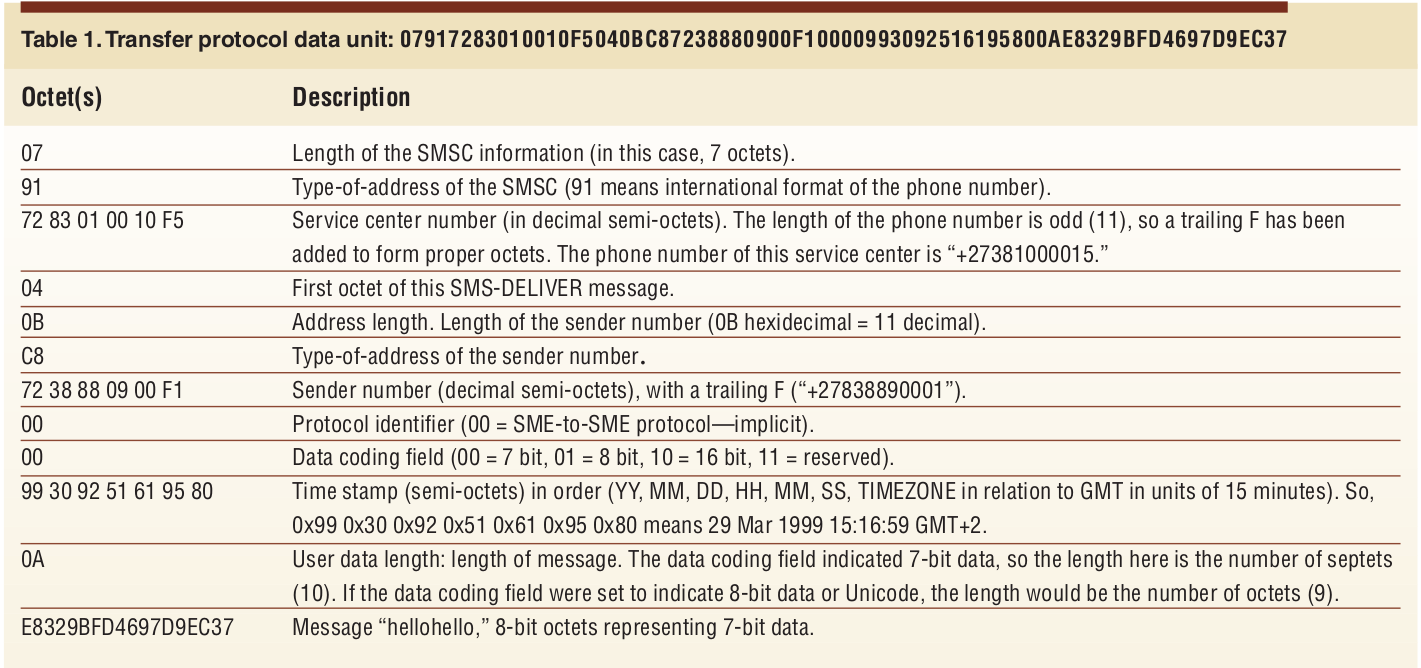
\includegraphics[width=0.9\textwidth]{img/tpdu-example.png}
		\label{tpdu-example}
	\end{figure}
\end{frame}

\begin{frame}{SMS-Architektur}
	\begin{figure}[htm]
		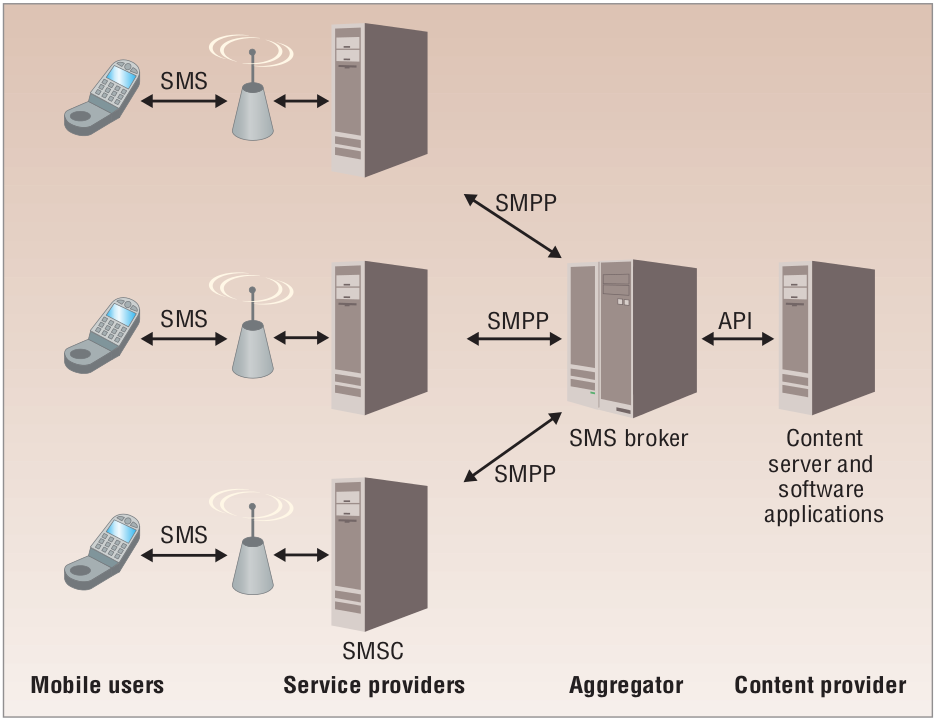
\includegraphics[width=0.7\textwidth]{img/sms-arch.png}
		\label{sms-arch}
	\end{figure}
\end{frame}

\begin{frame}{SMS-Versand -- Mobile Originated}

	\begin{tabular}{l l}
		\begin{minipage}{0.6\textwidth}
			\begin{itemize}
				\item Nachricht wird vom mobilen Endgerät über Funk zum Mobile Switching 
					Center/GRPS Core Network(VMSC/SGSN) geschickt
				\item VMSC/SGSN sendet mo-ForwardSM Operation an das zuständige SMSC 
					des Providers (Übermittlung von SMS-PP APDU)
				\item SMSC speichert Nachricht und versucht anschließend diese an die 
					Zieladresse auszuliefern
			\end{itemize}
		\end{minipage}
		&
		\begin{minipage}{0.4\textwidth}
			\begin{figure}[htm]
				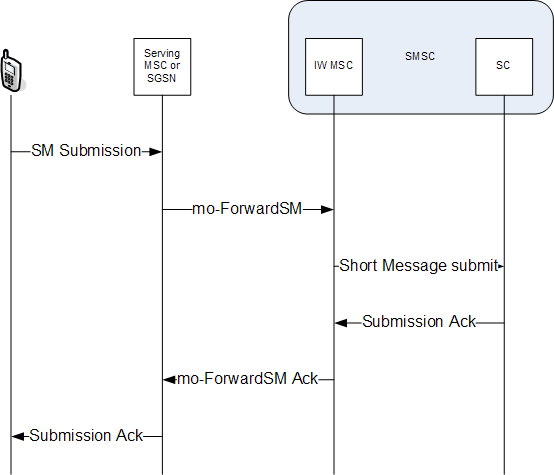
\includegraphics[width=\textwidth]{img/mo-forward-sm.png}
				\label{mo-forward-sm}
			\end{figure}	
		\end{minipage}
	\end{tabular}	
\end{frame}

\begin{frame}{SMS-Versand -- Mobile Terminated}

	\begin{tabular}{l l}
		\begin{minipage}{0.5\textwidth}
			\begin{itemize}
				\item SMSC sendet SMS-PP APDU der Nachricht an die Gateway MSC (GMSC) 
					Komponente des SMSC
				\item GMSC fragt beim Home Location Register (HLR) Position des 
					Empfängers an (SRI-for-SM)
			\end{itemize}
		\end{minipage}
		&
		\begin{minipage}{0.5\textwidth}
			\begin{figure}[htm]
				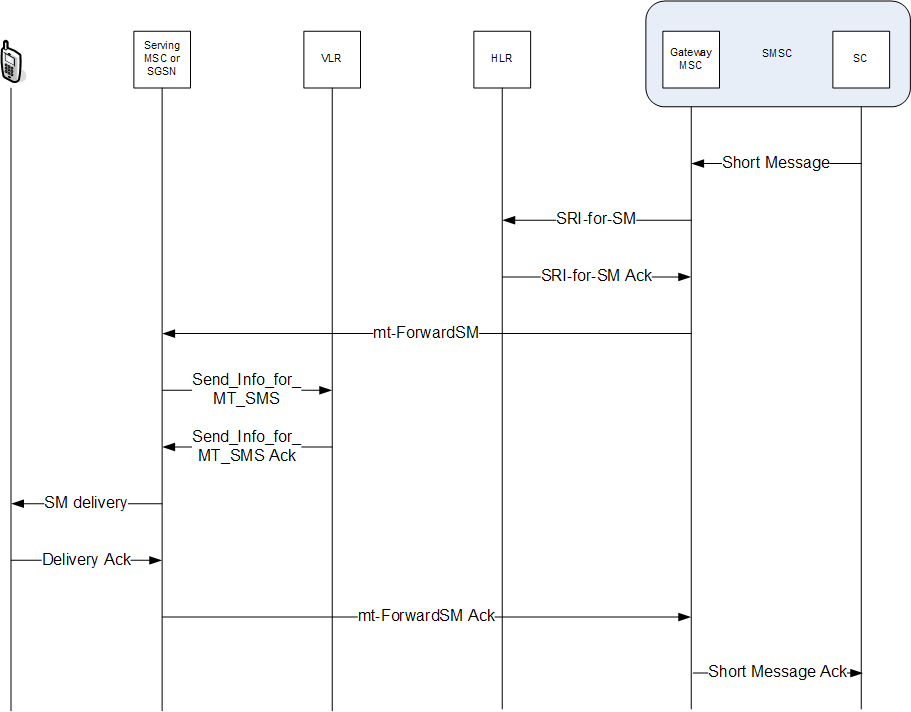
\includegraphics[width=\textwidth]{img/mt-forward-sm.png}
				\label{mt-forward-sm}
			\end{figure}	
		\end{minipage}
	\end{tabular}	
\end{frame}

\subsection{Nachteile}
\begin{frame}{Nachteile von SMS über GSM/GPRS}
	\begin{itemize}
		\item \textbf{Nicht Multi-Device tauglich}: SMS Service ist an eine einzige 
			Mobilfunknummer gebunden
		\item Kosten: SMS im Vergleich zu Kommunikation über Datennetz sehr 
			\textbf{teuer}
		\item \textbf{Keine Real-Time-Kommunikation} möglich; lange Zustellzeiten; 
			kein ``is typing''-Feature
		\item \textbf{Keine Gruppennachrichten} möglich
		\item Durch Limitation auf 160 7-Bit-Zeichen \textbf{keine Rich-Text-Nachrichten} 
			möglich
		\item Übertragungskanal ursprünglich nicht für das heutige 
			Nachrichtenaufkommen ausgelegt
	\end{itemize}
\end{frame}

\section{SMS über Datennetze}
\begin{frame}{Datennetzbasierte SMS Alternativen}
	\begin{itemize}
		\item Viele Alternativen zur herkömmlichen SMS
	\end{itemize}
	\begin{figure}[htm]
		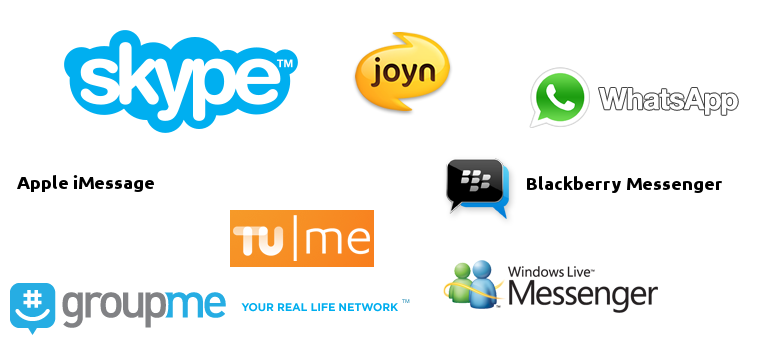
\includegraphics[width=\textwidth]{img/messengers.png}
		\label{messengers}
	\end{figure}
\end{frame}

\begin{frame}{RCS-e}
	\begin{itemize}
		\item Item 1
		\begin{itemize}
			\item Subitem 1
		\end{itemize}
		\item Item 2
		\item Item 3
	\end{itemize}
\end{frame}

\section{Ausblick}
\begin{frame}{Ausblick}
	\begin{itemize}
		\item Item 1
		\begin{itemize}
			\item Subitem 1
		\end{itemize}
		\item Item 2
		\item Item 3
	\end{itemize}
\end{frame}


\section{}

\begin{frame}{Quellen}	
	\scriptsize{
		\nocite{author1:title1,author1:title2}
		\bibliography{cites}
	}
\end{frame}


\begin{frame}
	\begin{center}
	\Huge{\textbf{Fragen?}}
	\end{center}
\end{frame}



\end{document}
